%%%%%%%%%%%%%%%%%%%%%%%%%%%%%%%%%%%%%%%%%%%%%%%%%%%%%%%%
%
% Change the option between square brackets
% depending on the document you have to write:
%
% proposal    for the initial proposal
% review      for the literature review
% progress    for the progress report
% final       for the final report
% 
%%%%%%%%%%%%%%%%%%%%%%%%%%%%%%%%%%%%%%%%%%%%%%%%%%%%%%%%
\documentclass[proposal]{cmpreport}
\makeatletter
%\input{t1pcr.fd}
\makeatother
\setlength{\footnotesep}{3ex}

% Some package I am using. You may not need them
%
\usepackage{rotating}
\usepackage{subfloat}

%\setkeys{Gin}{draft}

%%%%%%%%%%%%%%%%%%%%%%%%%%%%%%%%%%%%%%%%%%%%%%%%%%%%%%%%
%
%  Fill in the fields with:
%
%  your project title
%  your name
%  your registration number
%  your supervisor's name
%
%%%%%%%%%%%%%%%%%%%%%%%%%%%%%%%%%%%%%%%%%%%%%%%%%%%%%%%%
\title{Machine Learning competitions at Kaggle}

%%%%%%%%%%%%%%%%%%%%%%%%%%%%%%%%%%%%%%%%%%%%%%%%%%%%%%%%
%
% The author's name is ignored if the following command 
% is not present in the document
%
% Before submitting a PDF of your final report to the 
% project database you may comment out the command
% if you are worried about lack of anonimity.
%
%%%%%%%%%%%%%%%%%%%%%%%%%%%%%%%%%%%%%%%%%%%%%%%%%%%%%%%%
\author{Alan Lynch}


\registration{100094667}
\supervisor{Dr Gavin Cawley}
%%%%%%%%%%%%%%%%%%%%%%%%%%%%%%%%%%%%%%%%%%%%%%%%%%%%%%%%
%
% Fill in the field with your module code.
% this should be:
%
% for BIS            -> CMP-6012Y
% for BUSINESS STATS -> CMP-6028Y
% for other students -> CMP-6013Y
%
%%%%%%%%%%%%%%%%%%%%%%%%%%%%%%%%%%%%%%%%%%%%%%%%%%%%%%%%
\ccode{CMP-6013Y}


\summary{
A proposal of how to approach my third year project.
}

\acknowledgements{
This section is used to acknowledge who evers support and contribution.
The command that introduces it is ignored in the project proposal, literature review and progress report. It is used in the
final report,  but  is not compulsory. If you do not
have an acknowledgements command in your preamble then there
won't be any acknowledgement section in the document produced. \emph{Abstract} and \emph{Acknowledgements} sections should fit on the same page. 
}

%%%%%%%%%%%%%%%%%%%%%%%%%%%%%%%%%%%%%%%%%%%%%%%%%%%%%%%%%%%%%%%%%%
%
% If you do not want a list of figures and a list of tables
% to appear after the table of content then uncomment this line 
%
% Note that the class file contains code to avoid
% producing an empty list section (e.g list of figures) if the 
% list is empty (i.e. no figure in document).
%
% The command also prevents inserting a list of figures or tables 
% anywhere else in the document
%
% Some supervisors think that a report should not contain these
% lists. Please ask your supervisor's opinion.
%
%%%%%%%%%%%%%%%%%%%%%%%%%%%%%%%%%%%%%%%%%%%%%%%%%%%%%%%%%%%%%%%%%%
%\nolist

%%%%%%%%%%%%%%%%%%%%%%%%%%%%%%%%%%%%%%%%%%%%%%%%%%%%%%%%%%%%%%%%%%
%
% Comment out if you want your list of figures and list of
% tables on two or more pages, in particular if the lists do not fit 
% on a single page.
%
%%%%%%%%%%%%%%%%%%%%%%%%%%%%%%%%%%%%%%%%%%%%%%%%%%%%%%%%%%%%%%%%%%
\onePageLists

\linespread{1.5}

\begin{document}


\section{Introduction}
In this document I will outline the project I have undertaken, my aims, motivations, understanding of issues and problems that could be faced when working on the project, and highlight some key papers that may serve in improving my understanding of core topics surrounding my project. 
\section{Description of project}
The project I have undertaken is Machine learning competitions at Kaggle. In this project I will choose a competition from Kaggle.com and work towards submitting a solution to the competition, using machine learning techniques.
\subsection{Aims}
To submit a solution to a competition at Kaggle.com
\newline
To learn and understand core machine learning techniques
\newline
To be able to apply machine learning techniques to a real-world problem faced by a company.
\subsection{Motivations}
To gain a deeper understanding of machine learning techniques.
\newline
To gain an understanding of problems faced by companies.
\subsection{Understanding of issues}
Key issues include:
\begin{itemize}
	\item Reading through competitions list
    \item Highlighting potential competitions to enter
    \item Choosing a competition
    \item Familiarizing self with dataset
    \item Looking at machine learning papers that are relevant to the competition topics.
    \item Understanding core machine learning principles
    \item Implementing machine learning algorithms
    \item Applying machine learning algorithms to the competition dataset
    \item Computing / evaluate scores
    \item Improving algorithms and re-evaluating scores
    \item Repeating above two steps until highest score is achieved
\end{itemize}
\subsection{Problems}
Key problems include:
\begin{itemize}
	\item Problems with understanding of machine learning techniques
    \item Problems of applying machine learning techniques to competition dataset
    \item Problems evaluating algorithms
\end{itemize}
\section{Resources}
\subsection{Initial Reading}
The initial reading will be used to cover the fundamentals of Machine Learning.
Searching through goodreads.com shows a number of books that show potential:
\begin{itemize}
	\item Understanding Machine Learning: From Theory to Algorithms by Shai Shalev-Shwartz and Shai Ben-David
    \item Machine Learning by Tom M. Mitchell
    \item Machine Learning: A Probabilistic Perspective by Kevin P. Murphy
\end{itemize}
Less appropriate books that still may come into consideration include:
\begin{itemize}
\item Python Machine Learning by Sebastian Raschka
\item Machine Learning for Business Analytics by David Roi Hardoon, Galit Shmueli
\end{itemize}
\subsection{Papers}
Some popular papers worth reading include:
\begin{itemize}
\item ImageNet Classification with Deep Convolutional Neural Networks
\item Very deep convolutional networks for large-scale image recognition
\item Going Deeper with Convolutions
\item Deep Residual Learning for Image Recognition
\end{itemize}
More papers will be found once the competition has been chosen.
\section{Proposed approach}
My main idea for approaching the project would be to learn the basics of machine learning through the initial reading and make use of some on-line tutorials that may help reinforce the teachings of the books. Then planning how they might be used within the context of the competition dataset, and then reading through papers that look specifically at machine learning with datasets similar to the one I will be using. For example if the dataset is a collection of images, then it would be useful to look at machine learning papers that have data that is primarily images.
It would also be useful test out some of the techniques that had been learned with test data to see if the concepts had been learned / applied correctly. This would also give an opportunity for evaluating the effectiveness of the algorithms and give a chance for some optimization of the test algorithms, which will be useful when applying the algorithms to the competition dataset. Furthermore it would be good to get approval of the algorithms by my supervisor to ensure that I am on the right track.
Once tested, the algorithms (or some variation of them) could be applied to the competition dataset, evaluated, and then improved. Once I have a solution that both my supervisor and I deem suitable, it can then be submitted as a solution for the competition.

\section{Gantt Chart}
\begin{figure}[!htb]
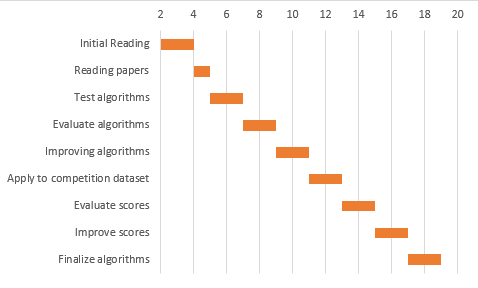
\includegraphics[]{project-gantt-chart.png}
\caption{A Gantt chart of tasks to be completed}
\end{figure}
\end{document}

